\documentclass[a4paper, 12pt]{article}%тип документа



%отступы
\usepackage[left=1cm,right=1cm,top=1cm,bottom=2cm,bindingoffset=0cm]{geometry}

%%% Работа с русским языком
\usepackage{graphicx}
\usepackage{cmap}                           % поиск в PDF
\usepackage{mathtext} 			 	       % русские буквы в формулах
\usepackage[T2A]{fontenc}               % кодировка
\usepackage[utf8]{inputenc}              % кодировка исходного текста
\usepackage[english,russian]{babel} 
\usepackage{float}

\usepackage[export]{adjustbox} % локализация и переносы

\usepackage{subfig}% http://ctan.org/pkg/subfig
\usepackage{booktabs}

\usepackage{wrapfig}


%Матеша
\usepackage{amsmath,amsfonts,amssymb,amsthm,mathtools} % AMS
\usepackage{icomma} % "Умная" запятая

%\mathtoolsset{showonlyrefs=true} % Показывать номера только у тех формул, на которые есть \eqref{} в тексте.

%% Шрифты
\usepackage{euscript}	 % Шрифт Евклид
\usepackage{mathrsfs} % Красивый матшрифт

%% Свои команды
\DeclareMathOperator{\sgn}{\mathop{sgn}}

%% Перенос знаков в формулах (по Львовскому)
\newcommand*{\hm}[1]{#1\nobreak\discretionary{}
	{\hbox{$\mathsurround=0pt #1$}}{}}


%\usepackage{caption}
%\usepackage{subcaption}

\date{18 октября 2022 г.}
\author{Гаврилин Илья Дмитриевич \\
	Б01-101}
\title{\textbf{Работа 3.4.2 \\ 
		Закон Кюри-Вейса}}
	
\begin{document}
	\maketitle
	\section{Аннотация}
	В работе изучили температурную зависимость магнитной восприимчивости ферромагнетика (гадолиний) выше точки Кюри. Определили значение температуры парамагнитной точки Кюри.
	\section{Теоретические сведения}
	Гадолиний является хорошим проводником электрического тока, a paбoчая частота генератора достаточно велика $(\sim 50$ к Гц $),$ поэтому для уменьшения вихревых токов образец изготовлен из мелких кусочков размером $\sim 0,5$ мм. Катушка 1 с образцом помещена в стеклянный сосуд 2, залитый трансформаторным маслом. 
	\begin{figure}
		\centering
		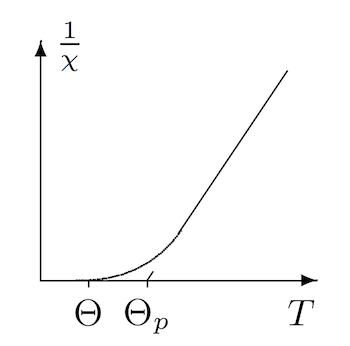
\includegraphics[width=0.3\linewidth]{graph}
		\caption{Теоретическая зависимость магнитной восприимчивости от температуры}
		\label{fig:graph}
	\end{figure}
	
	Масло предохраняет образец от окисления и способствует
	ухудшению электрического контакта между отдельными частичками образца. Кроме того, оно улучшает тепловой контакт между образцом и термостатируемой (рабочей) жидкостью 3 в термостате. Ртутный термометр 4 используется для приближённой оценки температуры.\\
	При изменении температуры меняется магнитная восприимчивость образца $\chi,$ а следовательно, самоиндукция катушки и период колебаний $\tau$ автогенератора. Для измерения периода используется частотомер.
	Закон Кюри Вейсса справедлив, если выполнено соотношение: 
	\begin{equation*}
		\frac{1}{\chi} \sim\left(T-\Theta_{p}\right) \sim \frac{1}{\left(\tau^{2}-\tau_{o}^{2}\right)}
	\end{equation*}
	
	где $\tau_{o}$ - период колебаний в отсутствие образца. Измерения проводятся в интервале температур от $12^{\circ} \mathrm{C}$ до $40^{\circ} \mathrm{C} .$ С целью
	экономии времени следует начинать измерения с низких температур.
	
	Для охлаждения образца используется холодная водопроводная вода, циркулирующая вокруг сосуда с рабочей жидкостью (дистиллированной водой); рабочая жидкость постоянно перемешивается.
	
	Величина стабилизируемой температуры задаётся на дисплее 5 термостата. Для нагрева служит внутренний электронагреватель, не показанный на
	рисунке.
	
	Когда температура рабочей жидкости в сосуде приближается к заданной, непрерывный режим работы нагревателя автоматически переходит в импульсный (нагреватель то включается, то выключается) - начинается процесс стабилизации температуры.
	
	Температура исследуемого образца всегда несколько отличается от температуры дистиллированной воды в сосуде. После того как вода достигла
	Заданной температуры, идёт медленный процесс выравнивания температур
	образца и воды. Разность их температур контролируется с помощью медноконстантановой термопары 6 и цифрового вольтметра. Один из спаев термопары находится в тепловом контакте с образцом, а другой погружён в воду. Концы термопары подключены к цифровому вольтметру. Рекомендуется измерять период колебаний автогенератора в тот момент, когда указанная разность температур становится $\leqslant 0,5^{\circ} \mathrm{C} .$ Чувствительность термопары $\mathrm{K}=24$ град $/ \mathrm{мB}$
	\section{Ход работы}
	1. Подождем охлаждения установки и термостата, дождемся стабилизации показаний частотомера.\\
	2. Дожидаясь момента когда разница между Температурой масла и воды станет $< 0.5 ~\%$. При этом записываем напряжение с учетом знака, для последующей корректировки температуры.\\
	\begin{equation*}
		T_{действ} = T_{термометр} + KU_{вольтметр},~ k= 24~град/мВ
	\end{equation*}
	3. Замерим показатели.\\
	\begin{table}[H]
		\centering
		\begin{tabular}{|l|l|l|l|l|}
			\hline
			$T, C^0$ & $\Delta U$, мВ & $T_{образца}, C^0$   & $\tau,$ мкс & $\tau^2 - \tau_0^2$, мкс \\ \hline
			14.15  & -0.005      & 14.03  & 8.0136     & 16.4807       \\ \hline
			16.11  & -0.015      & 15.75  & 7.9553     & 15.5497       \\ \hline
			18.1   & -0.017      & 17.692 & 7.8463     & 13.8273       \\ \hline
			20.1   & -0.017      & 19.692 & 7.6717     & 11.1179       \\ \hline
			22.08  & -0.016      & 21.696 & 7.4618     & 7.9414       \\ \hline
			24.09  & -0.015      & 23.73  & 7.2824     & 5.2963       \\ \hline
			26.08  & -0.018      & 25.648 & 7.2094     & 4.2384       \\ \hline
			28.09  & -0.017      & 27.682 & 7.1673     & 3.6331       \\ \hline
			30.09  & -0.011      & 29.826 & 7.1401     & 3.2439       \\ \hline
			32.07  & -0.017      & 31.662 & 7.1222     & 2.9886       \\ \hline
			34.07  & -0.017      & 33.662 & 7.1089     & 2.7994       \\ \hline
			36.06  & -0.018      & 35.628 & 7.0994     & 2.6644       \\ \hline
			38.06  & -0.019      & 37.604 & 7.0237     & 1.5953       \\ \hline
			40.04  & -0.017      & 39.632 & 7.0086     & 1.3834       \\ \hline
		\end{tabular}
		\caption{Экспериментальные данные}
	\end{table}
	4. Погрешности: Для погрешности частотомера имеем $\pm$ единицы последнего разряда, для итогового $\tau^2 - \tau_0^2$ получем погрешность $\pm 0.0002~мкс^2$, для температуры получим погрешность в среднем менее $< 0.5 \%$, точную укажем на графике.\\
	5. Построим зависимость $\frac{1}{\chi} = f(T)$\\
	\begin{figure}[H]
		\centering
		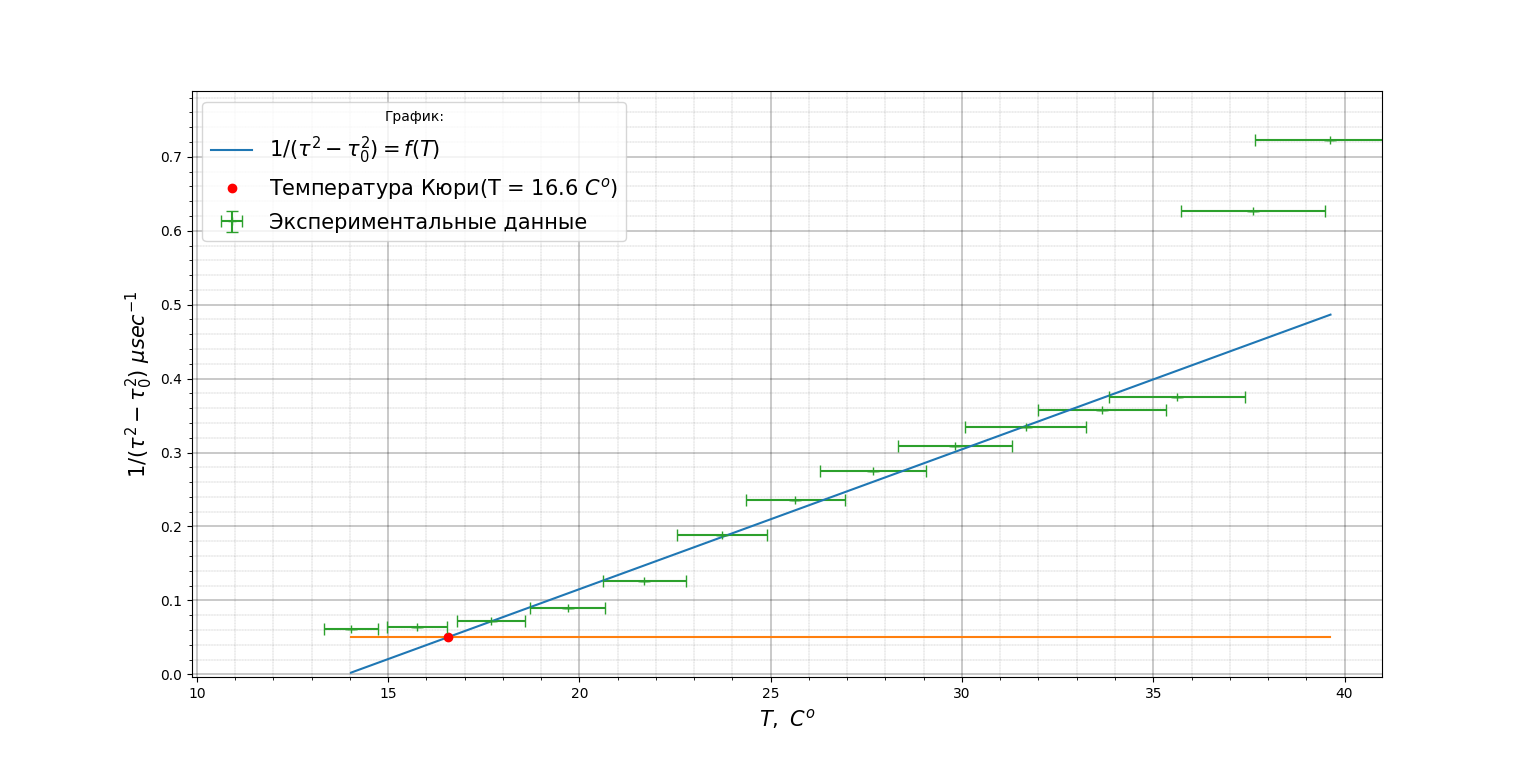
\includegraphics[width=0.9\linewidth]{temp}
		\caption{Зависимость $\frac{1}{\chi} = f(T)$}
		\label{fig:temp}
	\end{figure}
	По этой зависимости определили парамагнитную температуру Кюри, она оказалась равна:\\ $\Theta_p = (16.6\pm1.2)~C^o$.\\
	\section{Выводы}
	1. Проверили справедливость закона Кюри-Вейса, начиная с некоторой температуры Зависимость становится линейной.\\
	2. Нашли парамагнитную температуру Кюри: $\Theta_p = (16.6\pm1.2)~C^o$, она оказалась сходной с точкой Кюри: $T_k = 292~K$.\\
\end{document}